\documentclass[../../../main.tex]{subfiles}
\begin{document}
On s'est intéressé dans la première partie sur les graphes aux graphes non valués, c'est-à-dire pour lesquelles on n'associait pas de distances ni aucun autre genre de valeurs aux arcs.

On étend la définition d'un graphe orienté en ajoutant un valuation. On étend les représentations de même. On décrit de nouveaux algorithmes qui tiennent compte de cette valuation. On s'intéresse en particulier :
\begin{itemize}
	\item au calcul d'un arbre couvrant minimal d'un graphe
	\item au calcul du plus court chemin entre deux sommets d'un graphe
\end{itemize}
\subsection{Définition et représentations}
\definition{Graphe valué} {
	Un graphe valué sur un monoïde $(K, +, 0_K)$ est un triplet $G = (S, A, V)$ où $V:A\rightarrow K$ est une fonction de valuation qui à chaque arc associe une valeur dans le monoïde $(K, +, 0_K)$.

	Si $(u, v)\not\in A$, on a par convention $V((u, v)) = 0_K$\newline

	Le poids d'un chemin $x_0\rightarrow \dots \rightarrow x_k$ est $V(x_0, x_1)+ \dots + V(x_{k-1}, x_k)$.
}
\textbf{Interprétations :} Si $K$ est
\begin{itemize}
	\item $(\mathbb{N}, +, 0)$ ou $(\mathbb{R}, +, 0)$, le poids d'un chemin $\gamma = u\rightarrow^*v$ s'interprète comme la \textit{longueur} de $\gamma$
	\item $([0, 1], \times, 1)$, un poids s'interprète comme une probabilité de changement d'état entre deux sommets
	\item $(\mathcal{P}(\Sigma^*), \dot, \{\varepsilon\})$\footnote{où $\Sigma$ est un alphabet, $\varepsilon$ est le mot vide, et où pour tous $A, B\in \mathcal{P}(\Sigma^*), A\dot B = \{ab\ |\ a\in A \wedge b\in B\}$}, le poids d'un chemin est langage, et un graphe valué est un automate\footnote{Automate généralisé, car d'ordinaire, le poids d'un arc est simplement un singleton $\{a\}\subset \Sigma^1$}.
\end{itemize}
\textbf{Exemple pour comprendre :} Le choix le plus commun de monoïde est $(\mathbb{N}, +, 0)$.\newline
Le graphe suivant est valué sur ce monoïde :
\begin{center}
	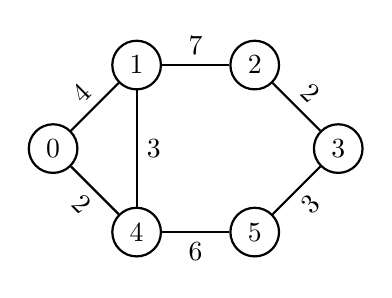
\begin{tikzpicture}[node distance={15mm}, thick, main/.style = {draw, circle}] 
	% Sommets :
	\node[main] (0) {$0$}; 
	\node[main] (1) [above right of=0] {$1$};
	\node[main] (2) [right of=1] {$2$};
	\node[main] (3) [below right of=2] {$3$};
	\node[main] (4) [below right of=0] {$4$};
	\node[main] (5) [right of=4] {$5$};
	% Arêtes
	\draw (2) -- node[midway, above, sloped] {7} (1);
	\draw (4) -- node[midway, right] {3} (1);
	\draw (4) -- node[midway, below, sloped] {2} (0);
	\draw (4) -- node[midway, below, sloped] {6} (5);
	\draw (2) -- node[midway, above, sloped] {2} (3);
	\draw (1) -- node[midway, above, sloped] {4} (0);
	\draw (3) -- node[midway, below, sloped] {3} (5);
	\end{tikzpicture} 
\end{center}
Le chemin $\gamma = 0\rightarrow 4 \rightarrow 1 \rightarrow 2 \rightarrow 3$ est de poids $2 + 3 + 7 + 2 = 14$. On peut donc dire que la longueur du chemin $\gamma$ entre $0$ et $3$ est $14$.\newline
On observe que le plus court chemin entre $0$ et $3$ est $0\rightarrow 4 \rightarrow 5 \rightarrow 3$ (de poids $11$) selon la relation d'ordre usuel sur $\mathbb{N}$. On appelle la longueur de ce plus court chemin la \textit{distance} entre $0$ et $3$.

Dans un graphe valué dans $\mathbb{N}$, on cherche généralement les chemins les plus courts, pour optimiser les déplacements.

Dans toute la suite, la valuation sera dans incluse dans $\mathbb{R}$.
\subsection{Signature du type abstrait}
On désigne par $Monoide$ le type abstrait associé au monoïde $(K, +, 0_K)$.

On étend la signature de graphe donnée dans la sous-section \ref{sub:signature_du_type_abstrait_graphe}. 

\textit{Graphe\textless Sommet, Monoide\textgreater} utilise \textit{Sommet}, \textit{Liste\textless Sommet\textgreater}, \textit{Entier}, \textit{Monoide} :
\begin{itemize}
	\item $poids(Graphe:G, Liste<Sommet>:l)\rightarrow Monoide$ renvoie le poids du chemin $l_1\rightarrow \dots \rightarrow l_n$ formé par les sommets de la liste $l$
\end{itemize}
\subsection{Représentations}
On enrichit ici les représentations de graphe données dans la sous-section \ref{sub:representations_graphe} en ajoutant la fonction de valuation du graphe évaluée sur chaque arc.
\subsubsection{Matrice par liste de successeurs}
On peut représenter un graphe valué $G = (S, A, V)$ par listes d'adjacence en enrichissant la structure de noeud de liste. On utilise une liste $Liste<Sommet, Poids>$ qui stocke à la fois les successeurs d'un sommet mais également le poids de l'arête. C'est-à-dire que pour tout $u\in S$, $succ(u) := \{(v, V(u, v))\ |\ u\rightarrow v\}$
\subsubsection{Matrice d'adjacence}
Dans le cas d'un graphe valué $G = (S, A, V)$ sur un monoïde $(K, +, 0_K)$, la matrice d'adjacence $M\in\mathcal{M}_{|S|}(K\cup\{\textit{NONE}\})$ représentant $G$ est telle que :
$$\forall (u, v)\in S\times S, M_{u, v} = \left\{\begin{array}{ll}
V((u, v)) & \text{si } (u, v)\in A \\
\textit{NONE} & \text{sinon}
\end{array}\right.$$
\textit{NONE} est simplement un symbole quelconque indiquant l'absence d'arc. On évite ainsi l'ambiguïté qui apparaît si on utilise $0_K$ à la place. Certains arcs peuvent en effet avoir comme valuation $0_K$.
\subsection{Premières propriétés}
\definition{Arbre couvrant minimal}{}
\subsection{Algorithmes de Kruskal et Prim}
L'objectif des algorithmes de Kruskal et de Prim est de calculer l'arbre couvrant minimal d'un graphe connexe.
\subsection{Algorithme de Floyd-Warshall}
\subsection{Bellman-Ford}
\subsection{Dijkstra}
\subsection{Exercices}
\end{document}